\documentclass[12pt]{article}

% Packages
\usepackage[utf8]{inputenc}
\usepackage{amsmath,amsfonts,amssymb}
\usepackage{geometry}
\usepackage{graphicx}
\usepackage{enumitem}
\usepackage{placeins}
\usepackage{hyperref}
\usepackage{listings}
\usepackage{xcolor}
\usepackage{caption}
\usepackage{comment}
\usepackage[normalem]{ulem}
\geometry{a4paper, margin=1in}
\newcommand{\kt}{\texttt{kthread }}
\newcommand{\ut}{\texttt{uthread }}



\begin{document}

\title{
    \textmd{\textbf{CS4210\\TinyFile}}\\
    \vspace{0.1in}\small{March 2024}\\
}
\author{
    \begin{tabular}[t]{cc}
        \textbf{Eduardo Rodríguez Sánchez} & \textbf{Alberto Molina Felipe} \\
        \texttt{esanchez63@gatech.edu} & \texttt{afelipe3@gatech.edu} \\
    \end{tabular}
}

\date{}
\maketitle

% **************************************************** OVERALL DESIGN
\section*{Overall Design}

\subsection*{Introduction}
\par In this project, we propose an implementation of a compressing service in a linux sistem. The service offers a compression mechanism through shared memory, which can be access from all other processes inside the system. This is achieved though an efficient implementation of a shared memory mechanims, which provides a circular buffer abstraction where processes can directly write data.

\par The architecture is analogous to the implementation of domains in Xen. The tinyfile service works like \texttt{Dom0}, while each instance of the library in the apps are the different domains. Tinifile offers a compressing service throught memory sharing, that allows the clients to request compression of different files.

\subsection*{The role of Tinyfile Service (\texttt{DomU})}
\par Just as Dom0 manages and controls access to hardware and orchestrates the operations of other virtualized domains, the Tinyfile Service acts as the central command authority, orchestrating the compression operations of multiple application library instances. This service manages the following tasks:

\begin{itemize}
    \item \textbf{Resource Allocation:} The Tinyfile service initializes by creating the required memory segments and setting up the primary message queue, `\texttt{/tinyservice}', at startup. These inter-process communication mechanisms facilitate communication between the server and applications. Through effective resource allocation, the service ensures that all processes have the necessary resources to work correctly.

    \item \textbf{Communication:} Utilizing message queues, the Tinyfile Service manages a complex communication protocol with client library instances. It processes messages of types \textit{Init}, for starting communication; \textit{Compress Request}, for file compression tasks; and \textit{End}, to signal the termination of requests from an application. This structured communication framework enables the Tinyfile Service to handle requests and manage the flow of information.
    
    \item \textbf{File Compression:} At the core of its functionality, the Tinyfile Service processes compression requests sent through the message queues. When receiving a \textit{Compress Request}, the service reads the shared memory segments to perform the requested file compression.
    
    \item \textbf{Quality of Service:} The Tinyfile Service implements QoS by prioritizing tasks based on number of request per process. Our strategy ensures fair access to resources and maintains system performance by dynamically adjusting to the workload demands of each application instance.
\end{itemize}


\section*{Role of Application Instances as Domains (\texttt{DomU})}
In our program architecture, each application instance with its linked Tinyfile library functions like an instance of \texttt{DomU} in the Xen virtualization platform. These instances represent the consumer domains that interact with the central Tinyfile Service (\texttt{Dom0}), using its functionalities for file compression. The key aspects and responsibilities of the application are:

\begin{itemize}
    \item \textbf{Utilization of Shared Memory:} Application instances utilize the shared memory segments established by the Tinyfile Service for writing file contents and reading compression results.
    \item \textbf{State Management and Synchronization:} Each application instance manages its state within the shared memory system, similar to how \texttt{DomU} instances maintain their state within the virtualized environment. This includes synchronization mechanisms like mutexes and condition variables to ensure exclusive access to shared resources, guaranteeing data integrity and preventing race conditions.
	\item \textbf{Synchronous Operations:} The library offers synchronous mode, where application instances wait for the compression task to complete before proceeding. This mode is suitable for scenarios where the subsequent operations depend on the completion of the compression task.
	\item \textbf{Asynchronous Operations:} The library also offers asynchronous mode, where application instances can proceed with other tasks without waiting for the compression task to finish. This non-blocking approach tries to emulate the non-blocking I/O operations in virtualized environments, allowing application instances to optimize their performance by parallel processing.
\end{itemize}

\subsection*{Message Queues}

\par At startup, the service creates the shared memory chunks given the arguments and the main message queue. Under the \texttt{'/tinyservice'} message queue library instances can push 3 type of messages:
\begin{itemize}
    \item \textbf{Init:} When the app calls \texttt{init\_communication()} a message is sent with the process identifier, with the intention of keeping track of all instances for quality of service.
    \item \textbf{Compress Request:} Every time an app wants to compress a file, this message serves as the request and it includes the pid to identify the request. 
    \item \textbf{End:} When the app calls \texttt{close\_communication()}, tells the service that this instance won't be making anymore requests.
\end{itemize}


\par Once a library instance send a compress request in the main message queue it waits in its own queue \texttt{'/<pid>'}. When the service responds to a request it will send a message in this individual queue with the information requires to start the shared memory communication. The message contains how many message chunks and their size.

\begin{figure}[h]
\centering
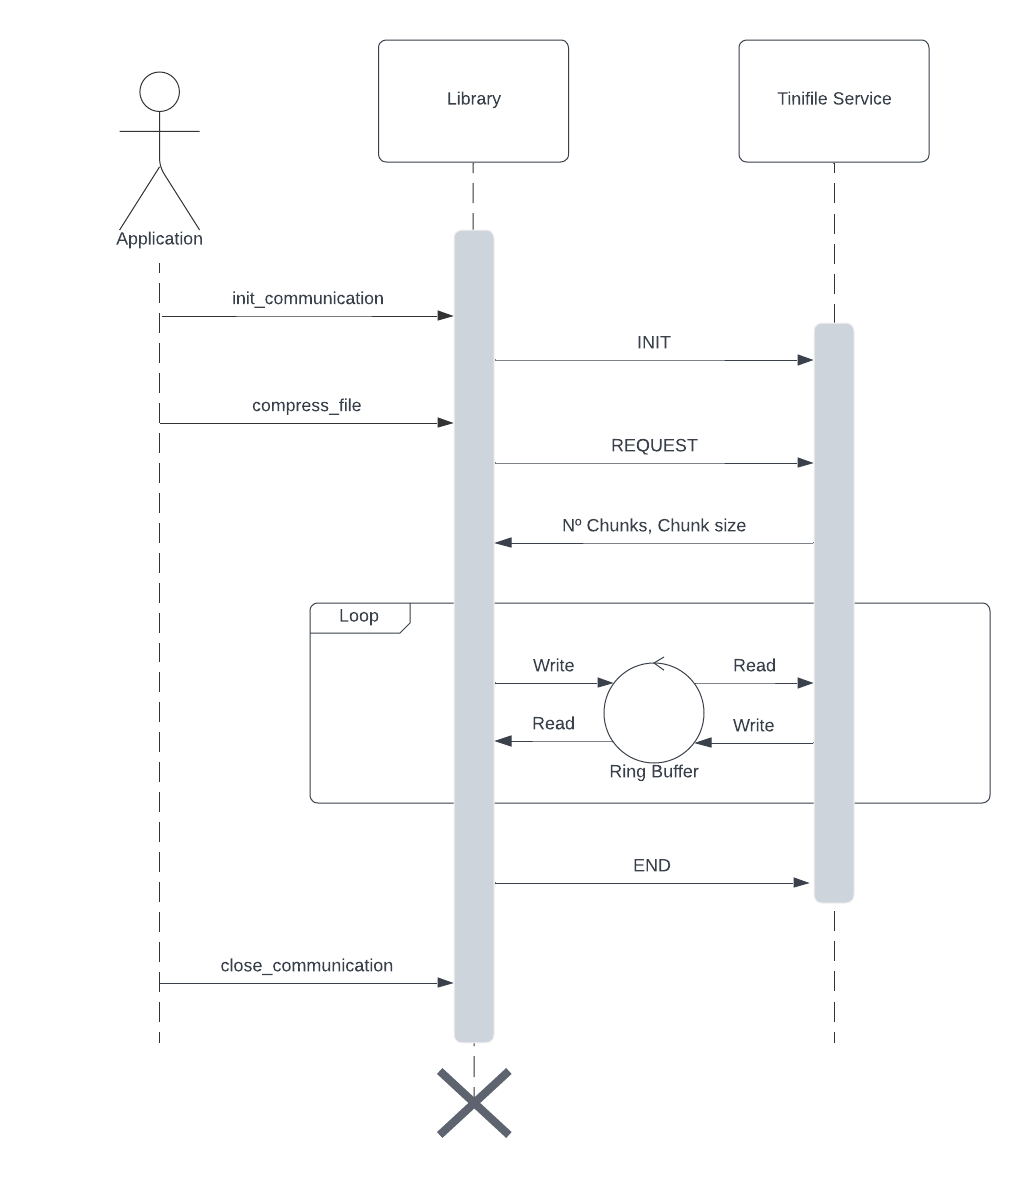
\includegraphics[width=\textwidth]{AOS-communication.png}
\end{figure}
\FloatBarrier
\newpage

\subsection*{Shared Memory}

\par At startup, the service allocates the shared memory chunks. Each chunk includes a mutex, condition variable, 2 integers and \texttt{sms\_size} bytes to communicate.

\par The mutex and condition variable serve a clear purpose, allow for exclusive access to the writable bytes in the chunk. The integers are specific to the tinyfile service.

\par The first integer in the chunk refers to the status and the other to the bytes written. We differentiated the possible contents of the chunk in raw/uncompressed data, compressed data and empty. Given those states the status of each chunk can be: \textit{empty}, \textit{raw}, \textit{compressed}, \textit{done\_lib} when its uncompressed and the library finished copying into shared memory and \textit{done\_ser} when its compressedand the service finished compressing the last chunk.

\par Communication with shared memory looks like a state machine. In the following table we describe the response of the library instance in each state. Its options are: read \texttt{R} or write \texttt{W} into the chunk, move to the next one \texttt{++} or hold on the mutex \texttt{H}.

\begin{table}[h]
\centering
\begin{tabular}{|l|c|c|c|c|c|}
\hline
\multicolumn{1}{|c|}{} & \multicolumn{5}{c|}{Chunk Status} \\ \hline
Library State & Empty & Raw & Compressed & Done Lib & Done Ser\\ \hline
Copying raw file & \texttt{W ++} & \texttt{H} & \texttt{R W ++}   & \texttt{-} & \texttt{-} \\
Finished copying & \texttt{++}   & \texttt{H} & \texttt{R ++}     & \texttt{H} & \texttt{R finish} \\ \hline
\end{tabular}
\end{table}


\par When it writes uncompressed bytes into the chunk it changes its status to \textit{raw}, if it happens to be its last chunk of bytes to write the status is changed to \textit{done\_lib} and it also signals how many bytes it has written, in case it doesn't fill the whole chunk.

\par The policy for the service is a lot simpler. It can hold, move one and compressed the chunks \texttt{Z}.When it compresses a chunk it always writes how many bytes it has written. If it compresses the chunk with status \textit{done\_lib} it 


\begin{table}[h]
\centering
\begin{tabular}{|c|c|c|c|c|}
\hline
\multicolumn{5}{|c|}{Chunk Status} \\ \hline
Empty & Raw & Compressed & Done Lib & Done Ser\\ \hline
\texttt{H} & \texttt{Z} & \texttt{H} & \texttt{Z finish} & \texttt{-} \\ \hline
\end{tabular}
\end{table}

\par We can illustrate some possible scenarios with the following diagrams. At first, the state of the shared memory array of chunks may look something like this. The library has written some raw chunks and the serviceis compressing the first chunk the library has written.

\begin{figure}[h]
\centering
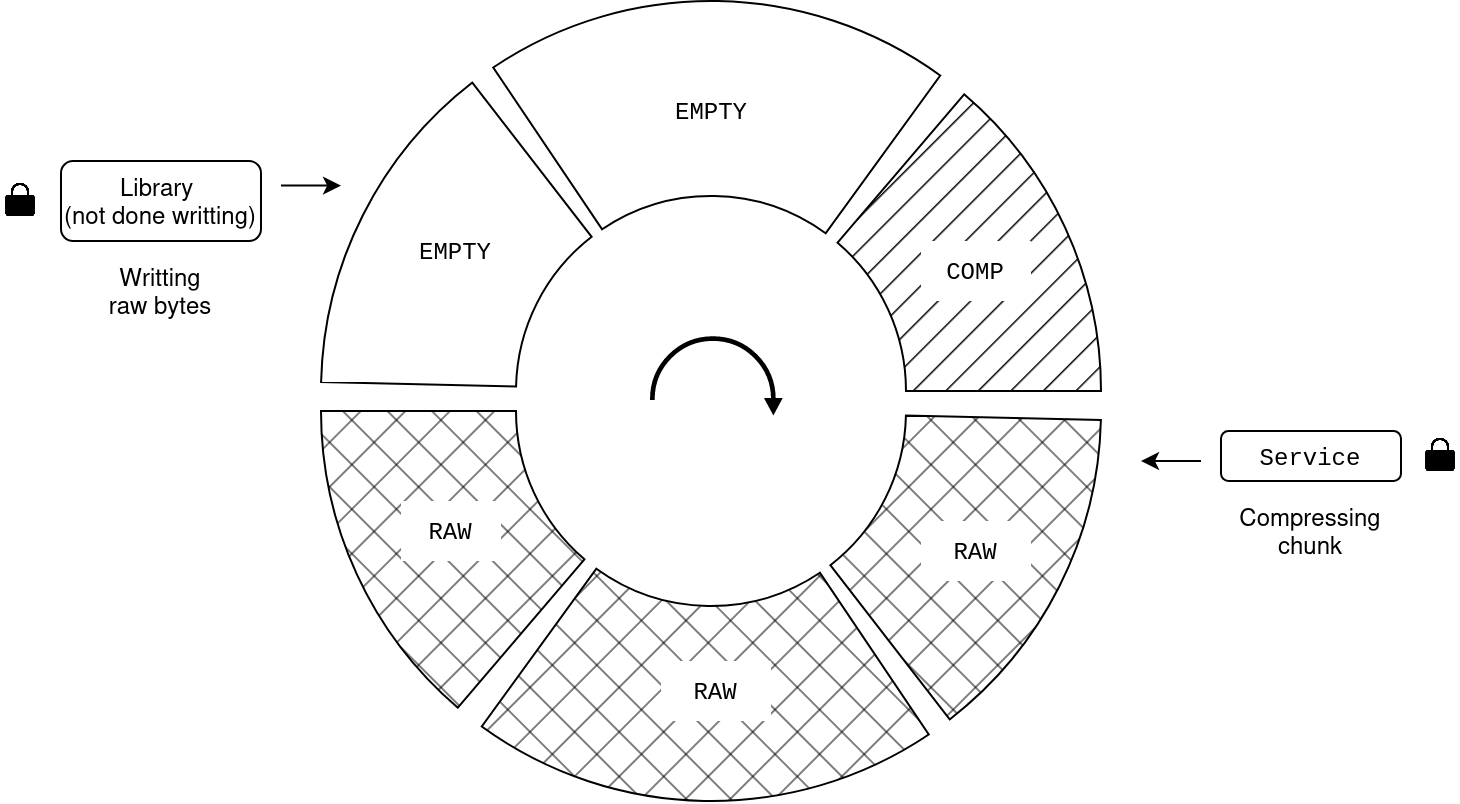
\includegraphics[width=0.6\textwidth]{AOS-start.png}
\end{figure}
\FloatBarrier

\newpage
\par In one scenario, the library had written its last raw chunk into the shared memory, and it moves to the first compressed chunk and copies its content to the output file. In this case, the service has taken longer to work around the circular buffer and has the mutex of the last chunk of raw bytes while the library has copied all the compressed bytes and is waiting to get the mutex.

\begin{figure}[h]
\centering
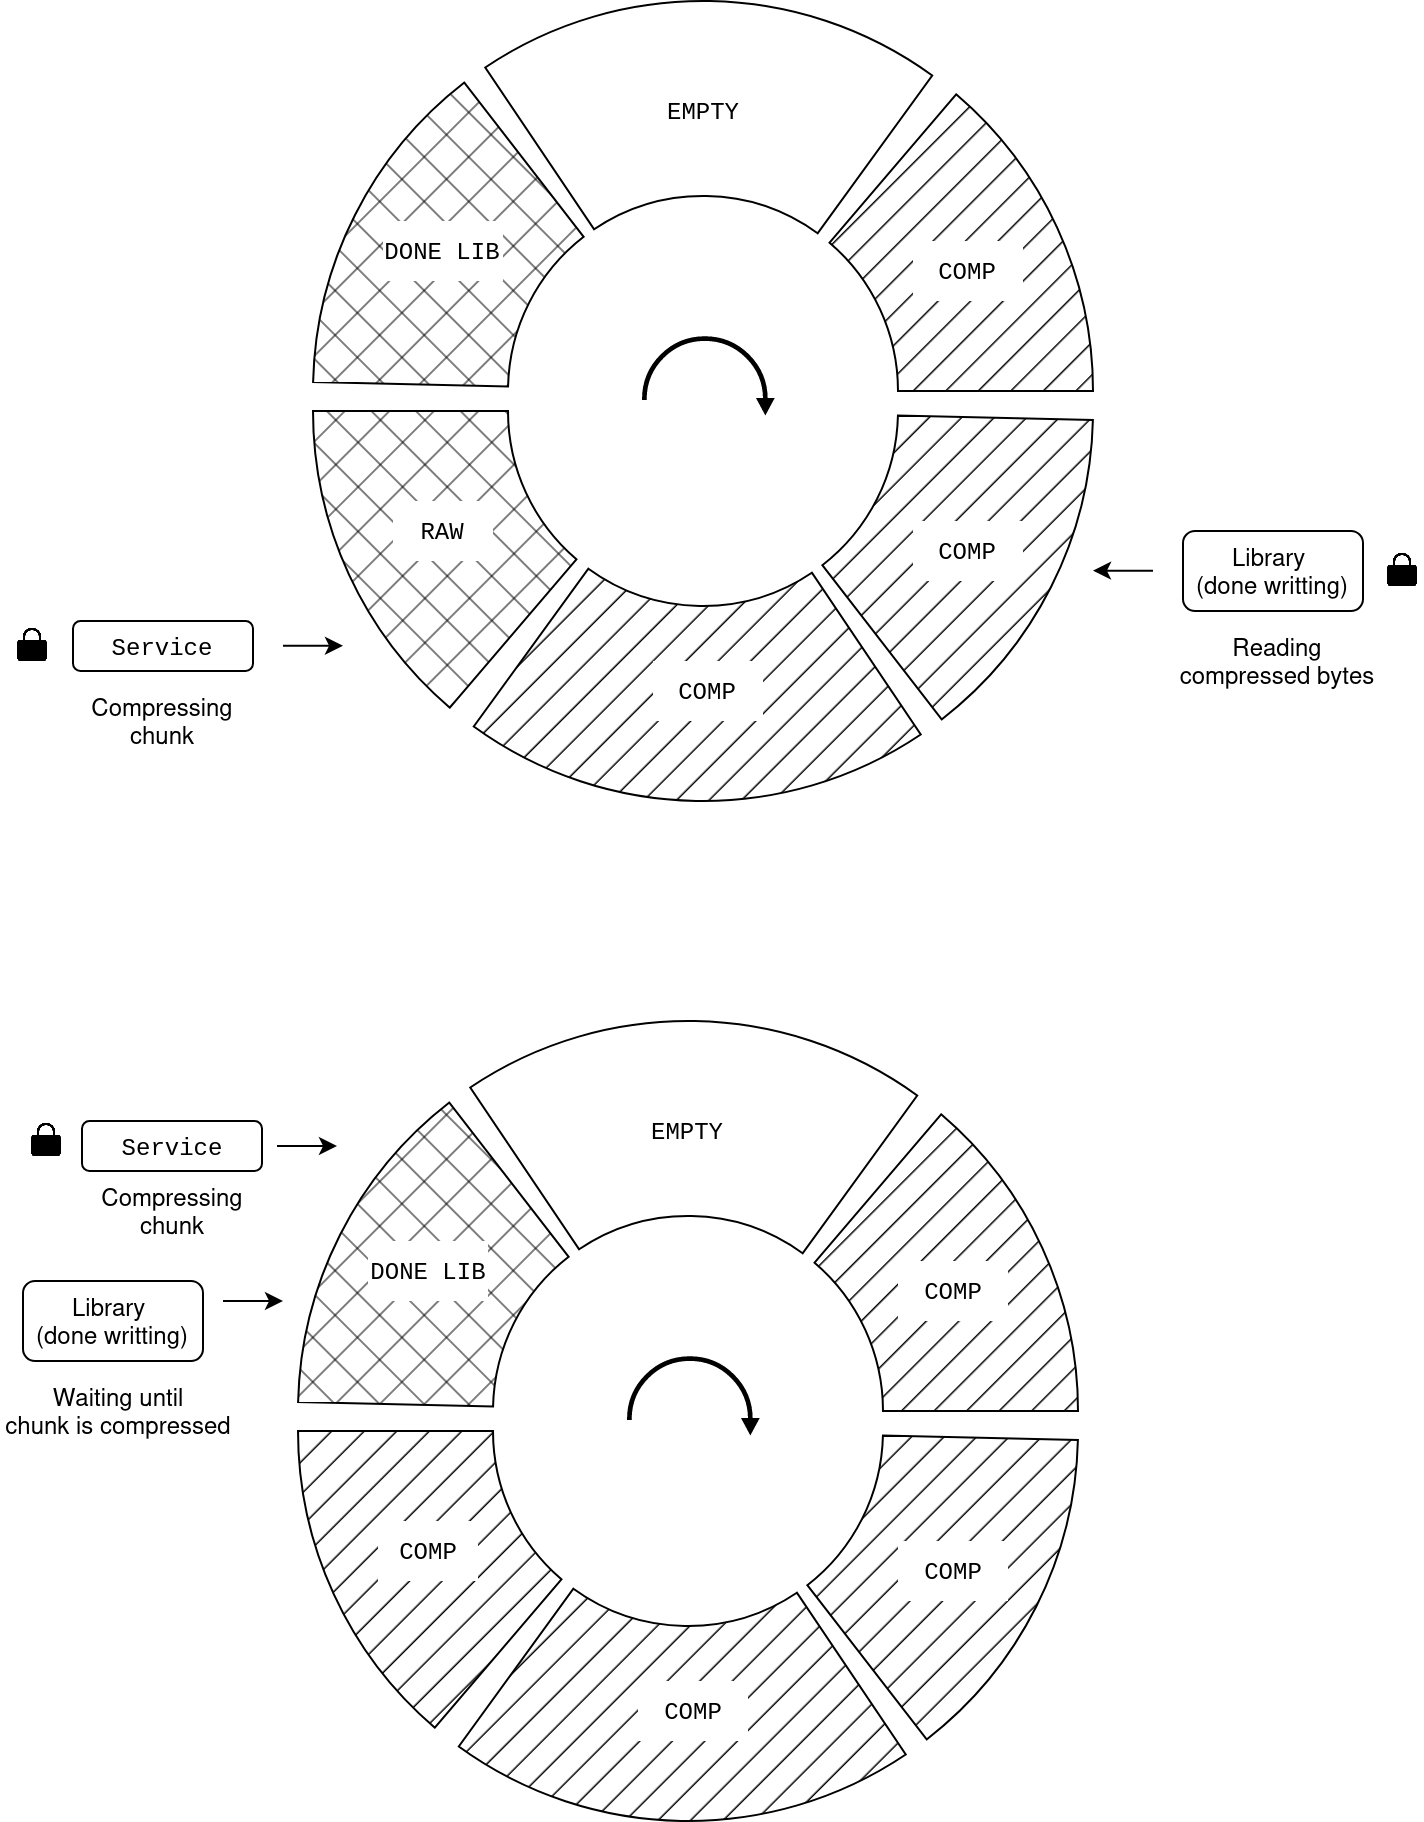
\includegraphics[width=0.9\textwidth]{AOS-done.png}
\end{figure}
\FloatBarrier


\newpage
\par In a second scenario, the library is compressing a larger file and it's not done copying the raw bytes.
The library has gone around each compressed chunk, reading its contents into the output file and writing the raw bytes.
Here, for scheduling or faster compression, the service has caught up to the library and is waiting on the mutex while the library is processing the compressed chunk.
\begin{figure}[h]
\centering
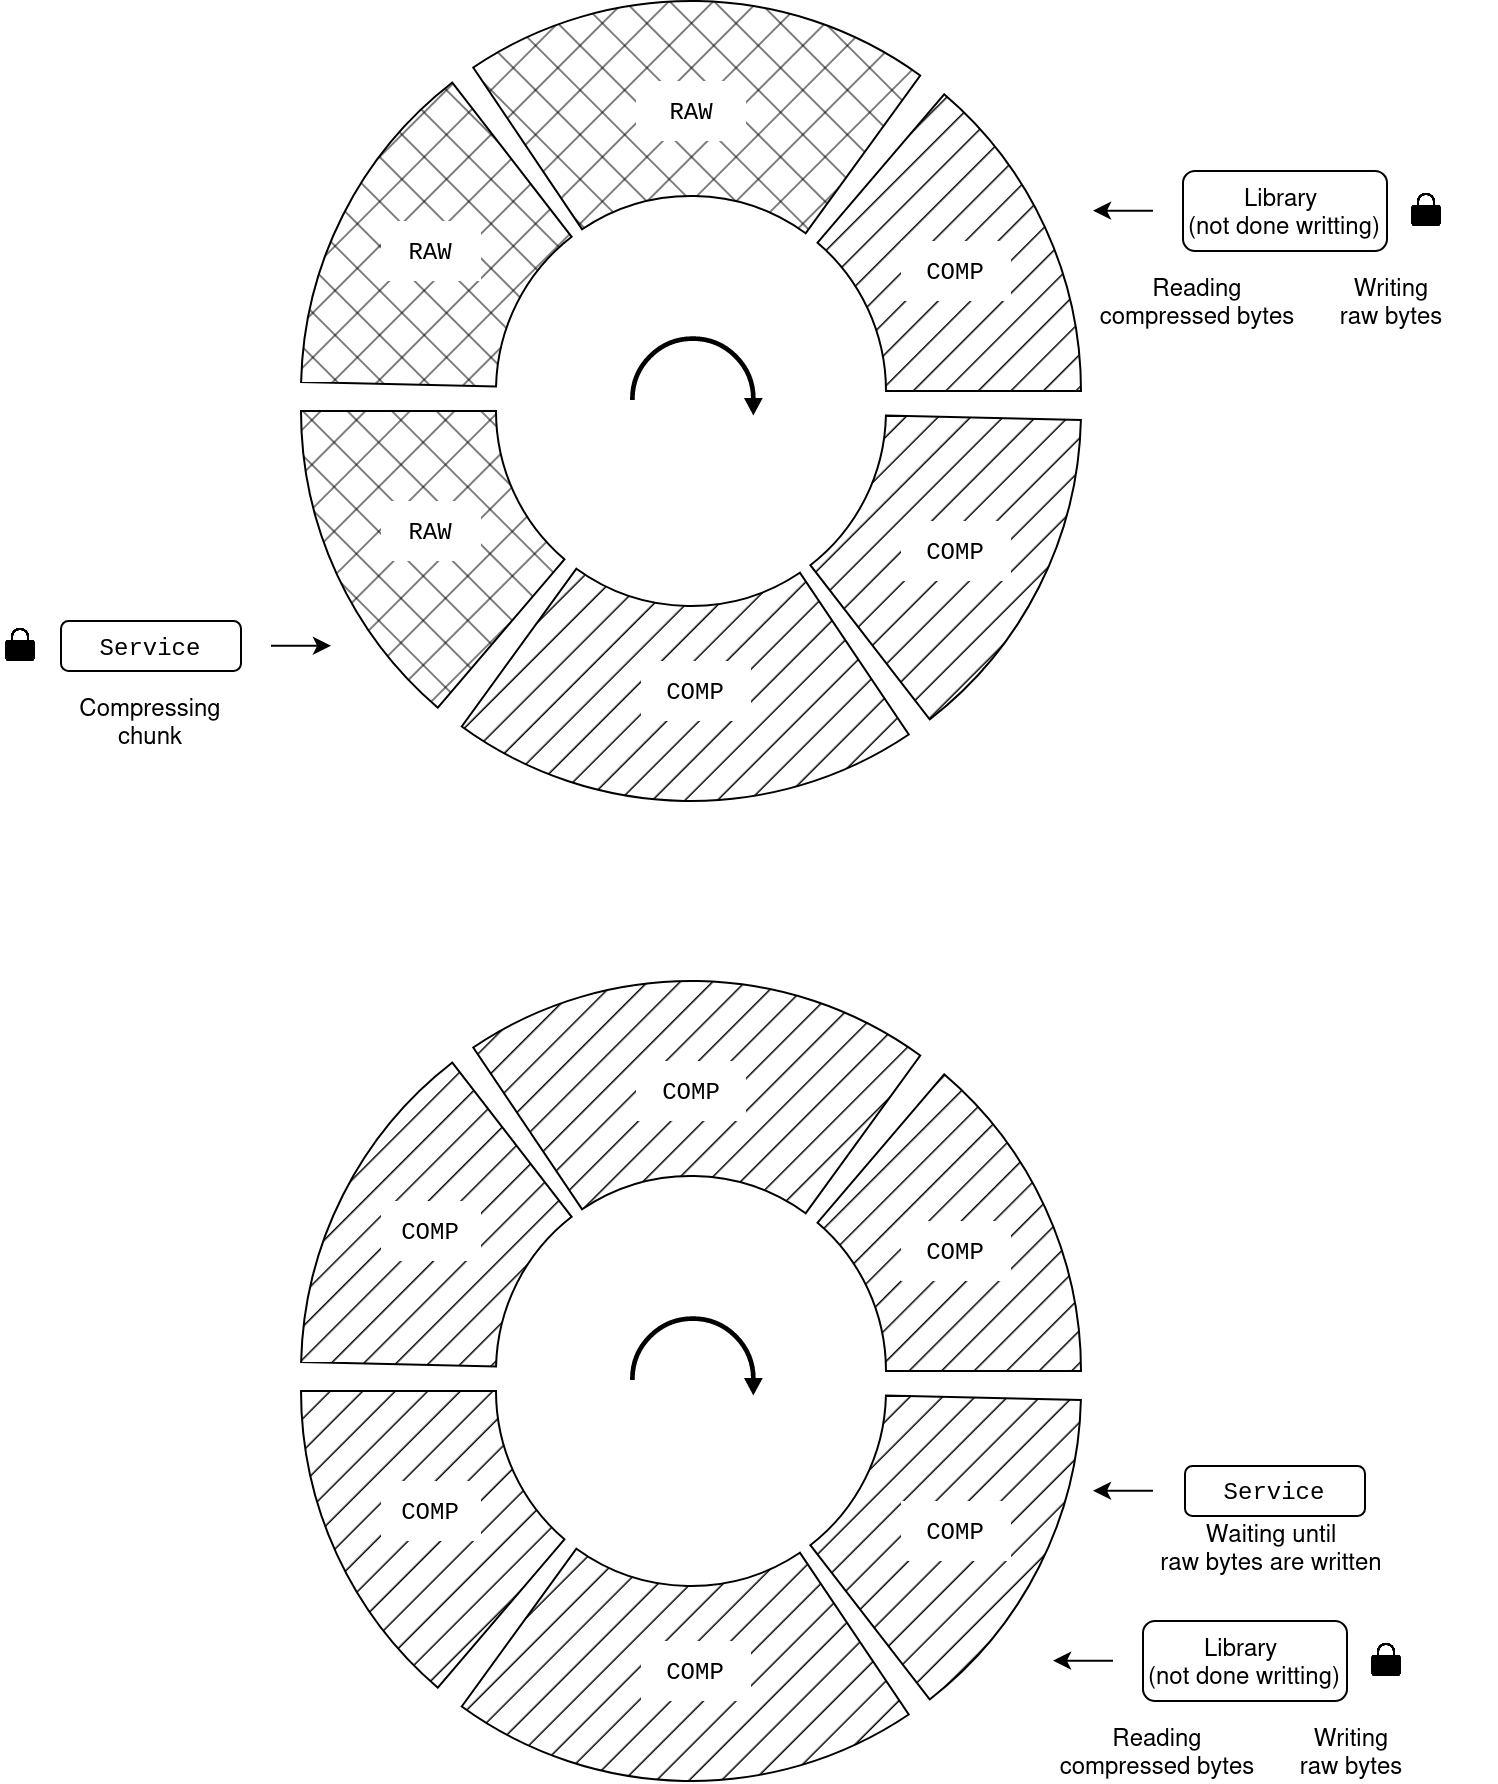
\includegraphics[width=0.9\textwidth]{AOS-not-done.png}
\end{figure}
\FloatBarrier
\newpage


% **************************************************** SYNC / ASYNC
\section*{Sync/Async Implementation}
In our system, we employ both synchronous and asynchronous mechanisms to handle data compression requests. By default, our system operates synchronously, executing a call-and-wait approach to data compressission. This means when a request is made to compress data, the system makes the necessary call to our compression service and halts operation, waiting the completion of the compression process. 

We have also implemented asynchronous calls to the compressing service. Asynchronous processing allows our system to initiate a compression request and then proceed with other operations without having to wait for the compression task to complete. This approach is particularly beneficial in high-performance environments where waiting on tasks could lead to significant inefficiencies. The asynchronous implementation involves modification of the core implementation:

\begin{itemize}
    \item \textbf{Wrapper Function:} We implemented a wrapper function that encapsulates the original synchronous compression call, so it can be assigned as a task to a thread.
    
    \item \textbf{Thread Launch:} For each compression request, a new thread is spawned that executes the wrapper function. This allows the main program to proceed with other tasks while the compression operation is carried out in a separate thread.
    
    \item \textbf{Synchronization Mechanism:} We use a structure containing a spinlock and a boolean variable named \textit{done} to manage the state of the asynchronous operation. The spinlock provides thread-safe access to the \textit{done} variable, indicating the completion status of the compression task, similar to what we would accomplish with an atomic variable.
    
    \item \textbf{Await Function:} An \textit{async\_await} function is implemented to monitor the completion of the compression task. This function checks the \textit{done} variable within the synchronization structure and waits for the compression task to finish and set \textit{done} to true.
\end{itemize}

% **************************************************** EXPERIMENT 
\section*{Experiment}



% **************************************************** QOS 
\section*{Quality of Service}
\par We implemented QoS in our project by prioritizing tasks based on the number of requests fulfilling. At first, we contemplated using a heuristic that accounts the number of bytes generated per process, but due to limitations of time we have considered only go with the simpler option of using number of request as the metric. Implementing QoS that accounts for byte consumption will be left as future work.

\par Starting the data exchange process with our service requires an initial communication phase where applications inform the server of their compression requirements. This is implemented through a system-initiated handshake, signaling the server of a new thread that wants a file compression.

\par Our service uses two diferent threads that handle request and compression (request thread and processing thread). The request thread reads the initial communication handshake and adds the process information to a linked list. Every time a process makes a request after the initial handshake, the request will be added into the queue of the corresponding node of the linked list. 

\par The processing thread iterates over the linked list, retrieving the first element of each node's queue and processing the request. It utilizes a round-robin approach so it ensures all processes are given a chance to get their requests fulfilled.

\par Using number of request per process as the heuristic, is implemented with the intent to democratize access to our services, ensuring the same amount of resources are distributed across all clients. By prioritizing tasks based on the number of requests, we acknowledge that we are leaving behind the consideration of data volume or the urgency of larger requests. Nevertheless, our primary objective remains to promote a balanced service across clients and to prevent Denial of Service attacks where a malicious client takes the entirety of the resources.
% **************************************************** LOGS
\section*{Logs}



% **************************************************** PRINTS
\section*{Figures}



\end{document}
